\section{Process}
\label{sec::chp5::process}

\begin{figure}[t]
\centering
\begin{tikzpicture}[
node distance=3.5cm,
block/.style={rectangle, rounded corners, draw, minimum width=2cm, minimum height=1.5cm},
queue/.style={rectangle, rounded corners, draw, minimum width=1cm, minimum height=0.8cm},
arrow/.style={->, thick}
]
% Generation stage
\node[block] (gen) {Password Generation};
% Queue
\node[queue, right of=gen] (queue) {Queue};
% Hashing stage
\node[block, right of=queue] (hash) {Hashing $\mu$};
% System boundary
\draw[dashed] ($(gen.north west)+(-0.2,0.2)$) rectangle ($(hash.south east)+(0.2,-0.2)$);
% Arrows
\draw[arrow] ($(gen.east)$) -- node[above] {$\lambda$} (queue.west);
\draw[arrow] (queue.east) -- node[above] {} (hash.west);
% System parameters
\node[below=0.8cm of queue] {System Utilization $\rho = \frac{\lambda}{\mu}$};
% Labels
\node[above=0.4cm of gen] {Stage 1};
\node[above=0.4cm of hash] {Stage 2};
% Optional explanation
% \node[below=1.5cm of hash, align=left, text width=20cm] 
%     {$\lambda$: Password candidate generation rate\\
%      $\mu$: Hash computation rate\\
%      $\rho$: System utilization};
\end{tikzpicture}
\caption{Visual representation of the password guessing process. Assuming an offline scenario where the attacker posses the hash value. $\lambda$ is password generation rate and arrival rate; $\mu$ is the hash rate or service rate; and $\rho$ is the utilization rate of the system.}
\label{fig:password-guessing-model}
\end{figure}

When attackers attempt to guess passwords, they must overcome hash functions that are designed to be computationally infeasible to invert (one-way function property). Therefore, we should naturally be interested in the rate at which they attempt this guessing. Whilst industry and the open-source community have focused on optimising hash rates to traverse the search space more quickly, academic literature and models have conversely neglected such optimisation. The question for us then is whether the newly proposed models perform better than even brute-force methods.

Systematising the guessing process provides a framework for optimising and allocating resources efficiently. By identifying bottlenecks, such as a slow dictionary generator, we can compare and select algorithms based on specific scenarios. Each stage in the process requires different resources, such as GPUs; therefore, modelling this process enables us to allocate these resources effectively. This systematic approach allows us to determine precisely how and when to scale or parallelise resources. Moreover, such a model helps to accurately determine both the cost and the time requirements for the entire process.

We model the password guessing process in two distinct steps: 1) Generation: This step produces a potential candidate for a given hash, and 2) Hashing: in this step, we compute the hash of the candidate password produced in the previous step. Whilst we assume that we are carrying out an offline attack (where we possess the hash value), this model can be generalised for other modes of attack. This process is visualised in Figure~\ref{fig:password-guessing-model}.

% \begin{axiom}[Offline Attack Assumption]
% Given a target hash value $h_t \in \{0,1\}^n$, the attacker has unrestricted access to $h_t$ and can compute $H(p)$ for any $p \in \mathcal{P}$.
% \end{axiom}
% 
% \begin{definition}[Password Guessing Process]
% Let $\mathcal{P}$ be the space of all possible passwords and $h: \mathcal{P} \rightarrow \{0,1\}^n$ be a cryptographic hash function. A password guessing process is a tuple $(G, H)$ where:
% \begin{itemize}
%     \item $G: \mathbb{N} \rightarrow \mathcal{P}$ is a generation function that produces candidate passwords
%     \item $H: \mathcal{P} \rightarrow \{0,1\}^n$ is the hash computation function
% \end{itemize}
% \end{definition}


%\begin{theorem}[Optimization Framework]
%The password guessing optimization problem can be formulated as:
%
%\[\min_{G} \{\mathbb{E}[X] \cdot \mathbb{E}[T]\}\]
%
%where $T$ is the random variable representing the time to generate and hash a single guess, subject to:
%\begin{enumerate}
%    \item $G$ must be computationally feasible
%    \item $\forall p \in \mathcal{P}, \exists i \in \mathbb{N}: G(i) = p$ (completeness)
%\end{enumerate}
%\end{theorem}
%
%\begin{definition}[Search Space Reduction]
%The efficiency of a generation function $G$ can be quantified by the search space reduction ratio:
%
%\[\rho(G) = \frac{|\{G(i): i \leq \mathbb{E}[X]\}|}{|\mathcal{P}|}\]
%
%where $\rho(G) \in (0,1]$ represents the fraction of the password space that must be explored before finding the target.
%\end{definition}


To optimise a password guessing algorithm, we need to balance two key factors:
\vspace*{-0.5cm}
\begin{enumerate}
    \item How well the algorithm guesses---measured by how many guesses it needs before succeeding. We can express this as $\mathbb{E}[X]$, where X represents the number of guesses.
    \vspace{-0.25cm}
    \item How quickly the algorithm generates its guesses. We measure this speed using $N(t)$, which represents the total guesses the algorithm has made by time t.
\end{enumerate}
% \begin{definition}[Guessing Efficiency]
% For a target password $p_t \in \mathcal{P}$ with hash $h_t = h(p_t)$, we define:
% \begin{itemize}
%     \item The number of guesses until success: $X = \min\{i: H(G(i)) = h_t\}$
%     \item The expected number of guesses: $\mathbb{E}[X]$
%     \item The guessing rate function: $N: \mathbb{R}^+ \rightarrow \mathbb{N}$, where $N(t)$ represents the cumulative number of guesses made by time $t$
% \end{itemize}
% \end{definition}

\subsection{Password Guessing Probability}

We will now incorporate the probability of successful guesses after a $x$ number of guesses guesses. Let $F(x)$ be the cumulative probability distribution function (CDF) of successful password guesses after $x$ number of guesses. $F(x)$ is essentially an assumed distribution by a guessing algorithm and we are interested in comparing these assumed distributions against each other with the ultimate aim of incorporating time (more on this in Section~\ref{how-passwords::time-to-crack}.)

\paragraph{Brute-force:}

The base case is a brute-force method that can be modelled using a uniform distribution. Let us assume the length of character space is $C$ and the length of a password is $\ell$. Our search space would therefore be $C^\ell$.

Uniform distribution for the brute-force method becomes:
\begin{equation}
    F_{\ell}(x) = \min \Bigl\{ \frac{x}{C^\ell},\,1 \Bigl\}
\end{equation}

Let $\mathcal{L}: \Omega \to \{1,\ldots,n\}$ be the random variable length. The composite distribution function becomes:

\begin{equation}
F_B(x) = \sum_{\ell=1}^n F_\ell(x) \, \mu_{\mathcal{L}}(\ell)
\end{equation}

where $\mu_{\mathcal{L}}$ is the probability mass function of password lengths. This then resolves to:

\begin{equation}
F_B(x) = \sum_{\ell=1}^n \min \Bigl\{ \frac{x}{C^\ell},\,1 \Bigl\} \, \mu_{\mathcal{L}}(\ell)
\end{equation}

% TODO: duplicated passwords
% Let $H = \{h_1, ..., h_k\}$ be a set of salted password hashes and $\mu_L: \mathbb{N} \to [0,1]$ be a password length distribution. The cumulative probability distribution function is:
% 
% $$
% F_B(x) = 1 - \prod_{i=1}^k \left(1 - \sum_{\ell \in \mathbb{N}} \min\left\{\frac{x}{C^\ell}, 1\right\} \mu_L(\ell)\right)
% $$
% 
% Taking the logarithm:
% 
% $$
% \log(1 - F_B(x)) = k \log\left(1 - \sum_{\ell \in \mathbb{N}} \min\left\{\frac{x}{C^\ell}, 1\right\} \mu_L(\ell)\right)
% $$
% 
% The expected number of guesses:
% 
% $$
% E[X] = \int_0^\infty \left(1 - \sum_{\ell \in \mathbb{N}} \min\left\{\frac{x}{C^\ell}, 1\right\} \mu_L(\ell)\right)^k dx
% $$
% 
% where:
% \begin{align*}
% k &: \text{number of salted hashes} \\
% C &: \text{character space size} \\
% \mu_L(\ell) &: \text{probability of length } \ell \\
% \sum_{\ell \in \mathbb{N}} \mu_L(\ell) &= 1
% \end{align*}

\paragraph{Logistic function:}

Based on the empirical results (as we shall see in Section~\ref{how-passwords::empirical-eval}), the deep learning models fit a logistic function well.
\begin{equation}
    F_L(x) = \frac{M}{1 + e^{-k(x-x_0)}}
\end{equation}
Where:
\begin{align*}
M & : \text{ maximum asymptotic value} \\
k & : \text{ logistic growth rate coefficient} \\
x_0  & : \text{ horizontal shift parameter (inflection point)} \\
\end{align*}

% \begin{equation}
% F(x) = 1 - e^{-(x/\eta)^\beta}
% \end{equation}
% \begin{equation}
% F(x) = A\,( 1 - e^{-bx} )
% \end{equation}
% where $\eta$ is the scale parameter and $\beta$ is the shape parameter.

\begin{figure}[t]
    \centering
    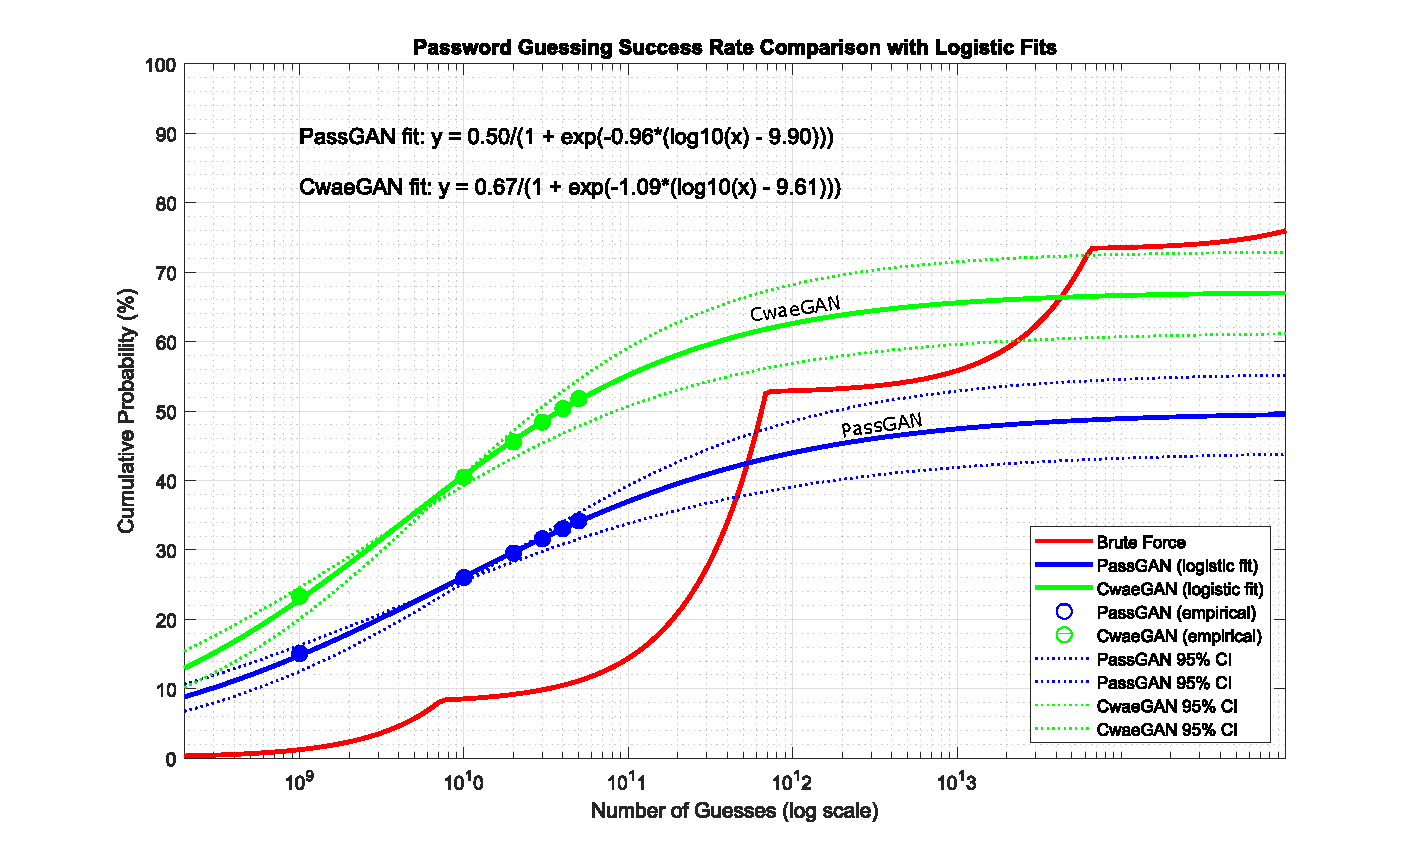
\includegraphics[scale=0.6]{figs/how_passwords/expected_guesses_chart2.pdf}
    \caption{Chart showing the cumulative probability distribution of \passgan, a similar GAN model (\cwaegan) and a brute-force method based on the Rockyou length distribution. The data fro the GAN models are taken from the same experiment and fitted with a logistic function. \srcOwnFig}
    \label{fig:password-expected-guesses}
\end{figure}

\subsection{Number of Guesses Empirical Evaluation}
\label{how-passwords::empirical-eval}

Putting our theoretical work into practice to this point, we want to ask how well the algorithms perform compared to the brute-force method. For this, we select the trawling attacks described in the \cwaegan and \omecdn papers.

For the length distribution $\mu_{\mathcal{L}}(\ell)$ (in brute-force method) we will use the empirical distribution from the Rockyou dataset as both papers used the RockYou password leak for training and testing their models, though they reported dataset details quite differently. The \omecdn paper provided comprehensive statistics, stating they used the Skullsecurity RockYou leak containing 32.6M passwords, which reduced to 14.3M after deduplication, and was further processed by removing passwords over 10 characters and those with illegal characters before being split 80:20 for training and testing. In contrast, the \cwaegan paper only briefly mentioned using the RockYou corpus with passwords up to 10 characters and filtered uncommon characters, but did not provide specific dataset sizes or train/test split details. This difference in dataset transparency makes it difficult to directly compare model performance.

We assume that models stop producing meaningful password candidates at some point and therefore the logistic function fits the empirical data well--as shown in Figure \ref{fig:password-expected-guesses}. The brute-force method overtakes the two GAN models in \cwaegan\ at $\sim4.7\times10^{13}$ guesses (68\% successful guesses). 
%%%%%%%%%%%%%%%%%%%%%%%%%%%%%%%%%%%%%%%%%%%%%%%%%%%%%%%%%%%%%%%%
\subsection{Expected Time to Crack}
\label{how-passwords::time-to-crack}
Let's assume the cumulative number of guesses made up to time $t$ is $N(t)$, therefore the cumulative probability of a successful guess by time $t$ is $F(N(t))$.  With this we can proceed to modelling the expected time to crack a password.
\begin{equation}
N(t) = \min(\lambda,\,\mu)\,t
\end{equation}
The system's performance metric combines both the queueing dynamics and success probability. The probability that the password is found in the interval $[t, t + dt]$ is $dF(N(t))$, so the expected time is:
\begin{equation}
\mathbb{E}[T_c] = \int_0^\infty t\,\frac{d}{dt}F(N(t))\,\di t = \int_0^\infty t\,f(N(t))\,N'(t)\,\di t
\end{equation}
To compute the expected time to successfully guess a password, we consider the time until a successful guess occurs, which depends on the number of processed guesses and their success probabilities. $N'(t) = \frac{dN(t)}{dt}$ is the rate at which the guesses are processed.

\paragraph{Uniform/Brute-force Function:}

\begin{multline*}
\\
\text{Starting with our CDF for brute-force:} \\
F_B(x) = \sum_{\ell=1}^n \min \Bigl\{ \frac{x}{C^\ell},\,1 \Bigr\} \, \mu_{\mathcal{L}}(\ell) \\
\end{multline*}
Evaluating the function with $N(t) = \min(\lambda, \mu)t$:
\begin{equation}
F_B(\min(\lambda, \mu)t) = \sum_{\ell=1}^n \min \Bigl\{ \frac{\min(\lambda, \mu)t}{C^\ell},\,1 \Bigr\} \, \mu_{\mathcal{L}}(\ell)
\end{equation}
This equation identifies the critical point where the ratio equals unity, representing the threshold condition for level $\ell$.
\begin{equation}
\frac{\min(\lambda, \mu)t}{C^\ell} = 1
\end{equation}
We define $T_\ell$ as the ratio of capacity at level $\ell$ to the minimum rate. This represents the time required to reach capacity at each level.
\begin{equation}
T_\ell = \frac{C^\ell}{\min(\lambda, \mu)}
\end{equation}
Substituting back:
\begin{equation}
\mathbb{E}[T_c] = \sum_{\ell=1}^n \mu_{\mathcal{L}}(\ell) \cdot T_\ell
\end{equation}
Finally:
\begin{equation}
\mathbb{E}[T_c] = \frac{1}{\min(\lambda, \mu)} \sum_{\ell=1}^n C^\ell \mu_{\mathcal{L}}(\ell)
\end{equation}

\paragraph{Logistic Function:}

Calculating the probability density function for our logistic CDF:
\begin{equation*}
F_L(x) = \frac{M}{1 + e^{-k(x-x_0)}}
\end{equation*}
\begin{equation*}
\text{Let } u = -k(x-x_0)
\end{equation*}
Substituting to simplify differentiation and using the chain rule:
\begin{equation*}
F(x) = M(1 + e^u)^{-1}
\end{equation*}
\begin{equation*}
\frac{dF}{du} = M \cdot (-1)(1 + e^u)^{-2} \cdot e^u
\end{equation*}
\begin{equation*}
\frac{du}{dx} = -k
\end{equation*}
Multiplying the derivatives:
\begin{equation*}
\frac{dF}{dx} = M \cdot (-1)(1 + e^u)^{-2} \cdot e^u \cdot (-k)
\end{equation*}
Simplifying:
\begin{equation*}
\frac{dF}{dx} = Mk \cdot \frac{e^u}{(1 + e^u)^2}
\end{equation*}
Final probability density function:
\begin{equation}
f_L(x) = Mk \cdot \frac{e^{-k(x-x_0)}}{(1 + e^{-k(x-x_0)})^2}
\end{equation}

\begin{figure}[ht]
    \centering
    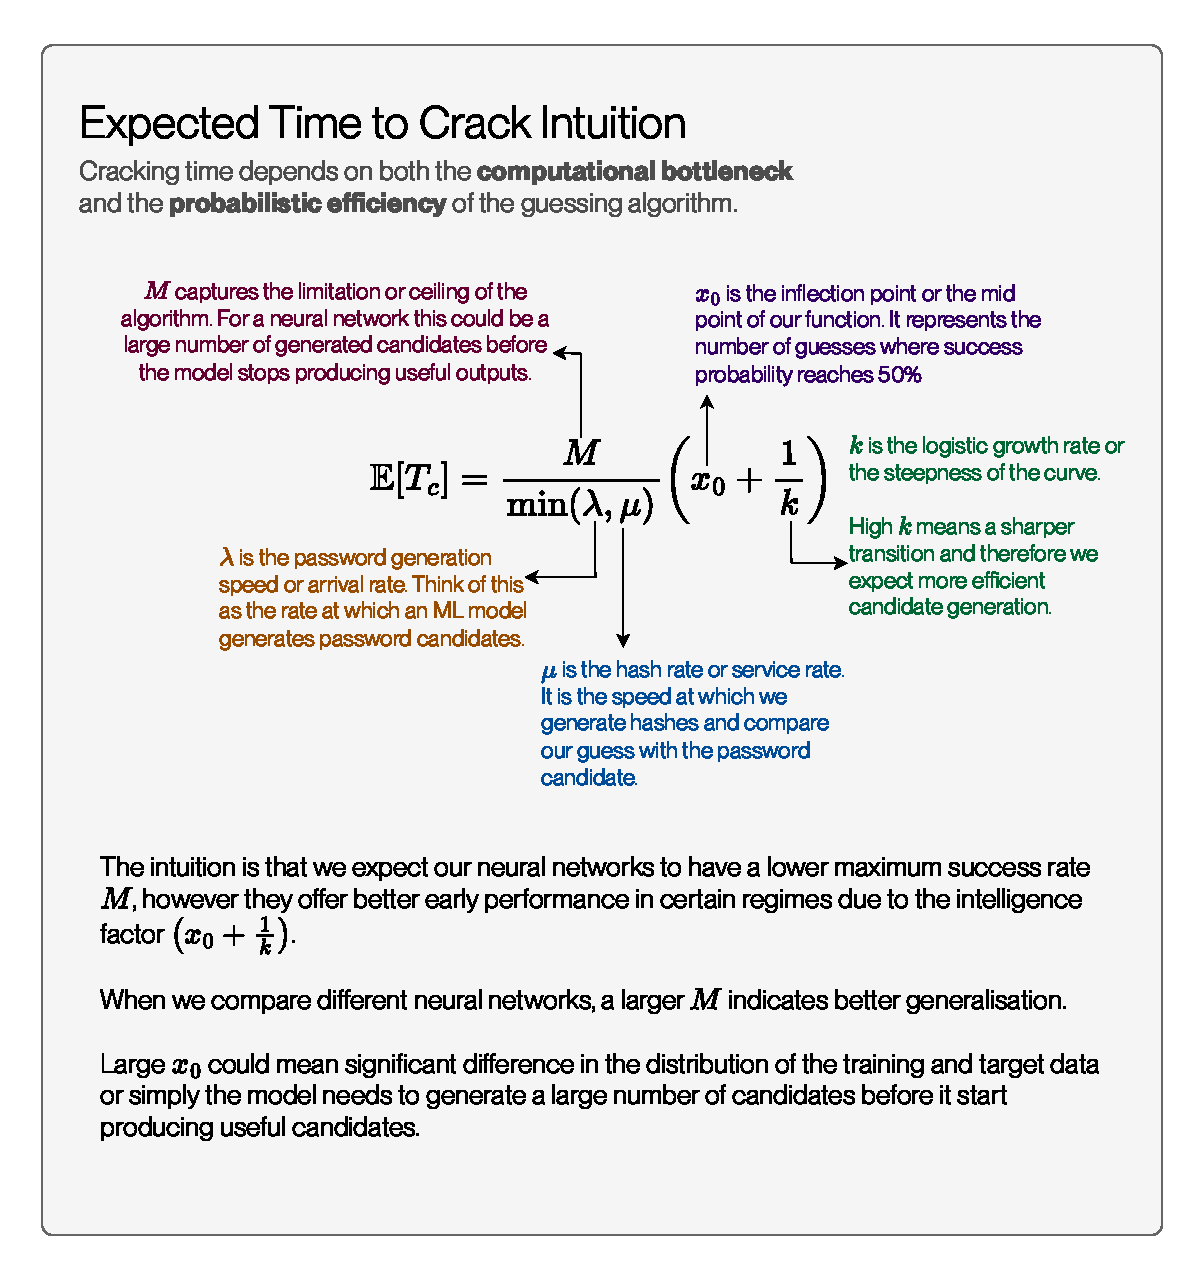
\includegraphics[width=0.7\linewidth]{figs//how_passwords/phd_equation.pdf}
    \caption{Visualisation of Equation~\ref{eq::515}. This figure explains the variables and provides some intuition behind the equation.}
    \label{fig::chp5::e_t_crack}
\end{figure}

Now we can calculate the expected Time to Crack for our logistic function:
\begin{align*}
\mathbb{E}[T_c] & = \int_0^\infty t \cdot \frac{kM\alpha e^{-k(\alpha t - x_0)}}{(1 + e^{-k(\alpha t - x_0)})^2}\,dt \\
& = \int_{-x_0}^\infty \frac{u + x_0}{\alpha} \cdot \frac{kM\alpha e^{-ku}}{(1 + e^{-ku})^2} \cdot \frac{du}{\alpha} \\
& = M\int_{-x_0}^\infty \frac{(u + x_0)ke^{-ku}}{(1 + e^{-ku})^2}\,du \\
& = M\left[\frac{x_0}{\alpha} + \frac{1}{k\alpha}\right] \\
\end{align*}
Our final equation then becomes:
\begin{equation}
\mathbb{E}[T_c] = \frac{M}{\min(\lambda, \mu)}\left(x_0 + \frac{1}{k}\right)
\label{eq::515}
\end{equation}

Equation~\ref{eq::515} shows the expected time to crack a password. $\lambda$ represents our arrival rate (or the number of password guesses we generate using a model), whilst $\mu$ is the hashing rate (or how many password hashes we can generate per unit of time). So, $\min(\lambda, \mu)$ tells us by what our system is throttled and is the \textit{effective} password guessing rate. Together, the expression $\left(x_0 + \frac{1}{k}\right)$ scales the basic time estimate $\frac{M}{\min(\lambda, \mu)}$ to account for both initial search conditions and the probabilistic nature of password discovery. This gives us a more realistic expected completion time that reflects both the computational constraints and the stochastic aspects of the guessing process. Figure~\ref{fig::chp5::e_t_crack} provides a detailed breakdown of the equation in visual form.

% TODO: Weibull distribution for expected guesses.
%\paragraph{Weibull distribution:}
%
%Substituting $f(N(t))$ and $N'(t)$, we get:
%\[
%E[T] = \int_0^\infty t \, \frac{\beta}{\eta} \left( \frac{N(t)}{\eta} \right)^{\beta - 1} e^{-(N(t)/\eta)^\beta} N'(t) \, dt.
%\]
%
%In cases where $N(t) = \nu t$, with $\nu = \min\{\lambda, \mu\}$, we have $N'(t) = \nu$, and $N(t) = \nu t$, so:
%\[
%E[T] = \int_0^\infty t \, \frac{\beta \nu^\beta}{\eta^\beta} t^{\beta - 1} e^{-(\nu t / \eta)^\beta} dt.
%\]
%
%Simplifying:
%\[
%E[T] = \frac{\beta \nu^\beta}{\eta^\beta} \int_0^\infty t^\beta e^{-(\nu t / \eta)^\beta} dt.
%\]
%
%Letting $u = \left( \frac{\nu t}{\eta} \right)^\beta$, we have:
%\[
%t = \frac{\eta}{\nu} u^{1/\beta}, \quad dt = \frac{\eta}{\nu} \frac{1}{\beta} u^{(1/\beta) - 1} du.
%\]
%
%Substituting back, we get:
%\[
%E[T] = \frac{\beta \nu^\beta}{\eta^\beta} \cdot \frac{\eta}{\nu} \cdot \frac{1}{\beta} \int_0^\infty \left( \frac{\eta}{\nu} u^{1/\beta} \right)^\beta u^{(1/\beta) - 1} e^{-u} du.
%\]
%
%Simplifying, the integrand becomes:
%\[
%\left( \frac{\eta}{\nu} u^{1/\beta} \right)^\beta = \left( \frac{\eta}{\nu} \right)^\beta u.
%\]
%
%Therefore, the expected time simplifies to:
%\[
%E[T] = \frac{\nu^\beta}{\eta^\beta} \cdot \frac{\eta}{\nu} \cdot \left( \frac{\eta}{\nu} \right)^\beta \int_0^\infty u e^{-u} du = \frac{\eta}{\nu} \Gamma(2),
%\]
%where $\Gamma(2) = 1! = 1$.
%
%Thus, the expected time to find the password is:
%\[
%E[T] = \frac{\eta}{\nu}.
%\]
%
%However, this result holds for $\beta = 1$, which corresponds to the exponential distribution. For a general $\beta$, the expected number of guesses is:
%\[
%E[N] = \eta \Gamma\left(1 + \frac{1}{\beta}\right),
%\]
%so the expected time to find the password is:
%\[
%E[T] = \frac{E[N]}{\nu} = \frac{\eta}{\nu} \Gamma\left(1 + \frac{1}{\beta}\right).
%\]
\subsection{Time to Crack Empirical Evaluation} 

\begin{figure}
    \centering
    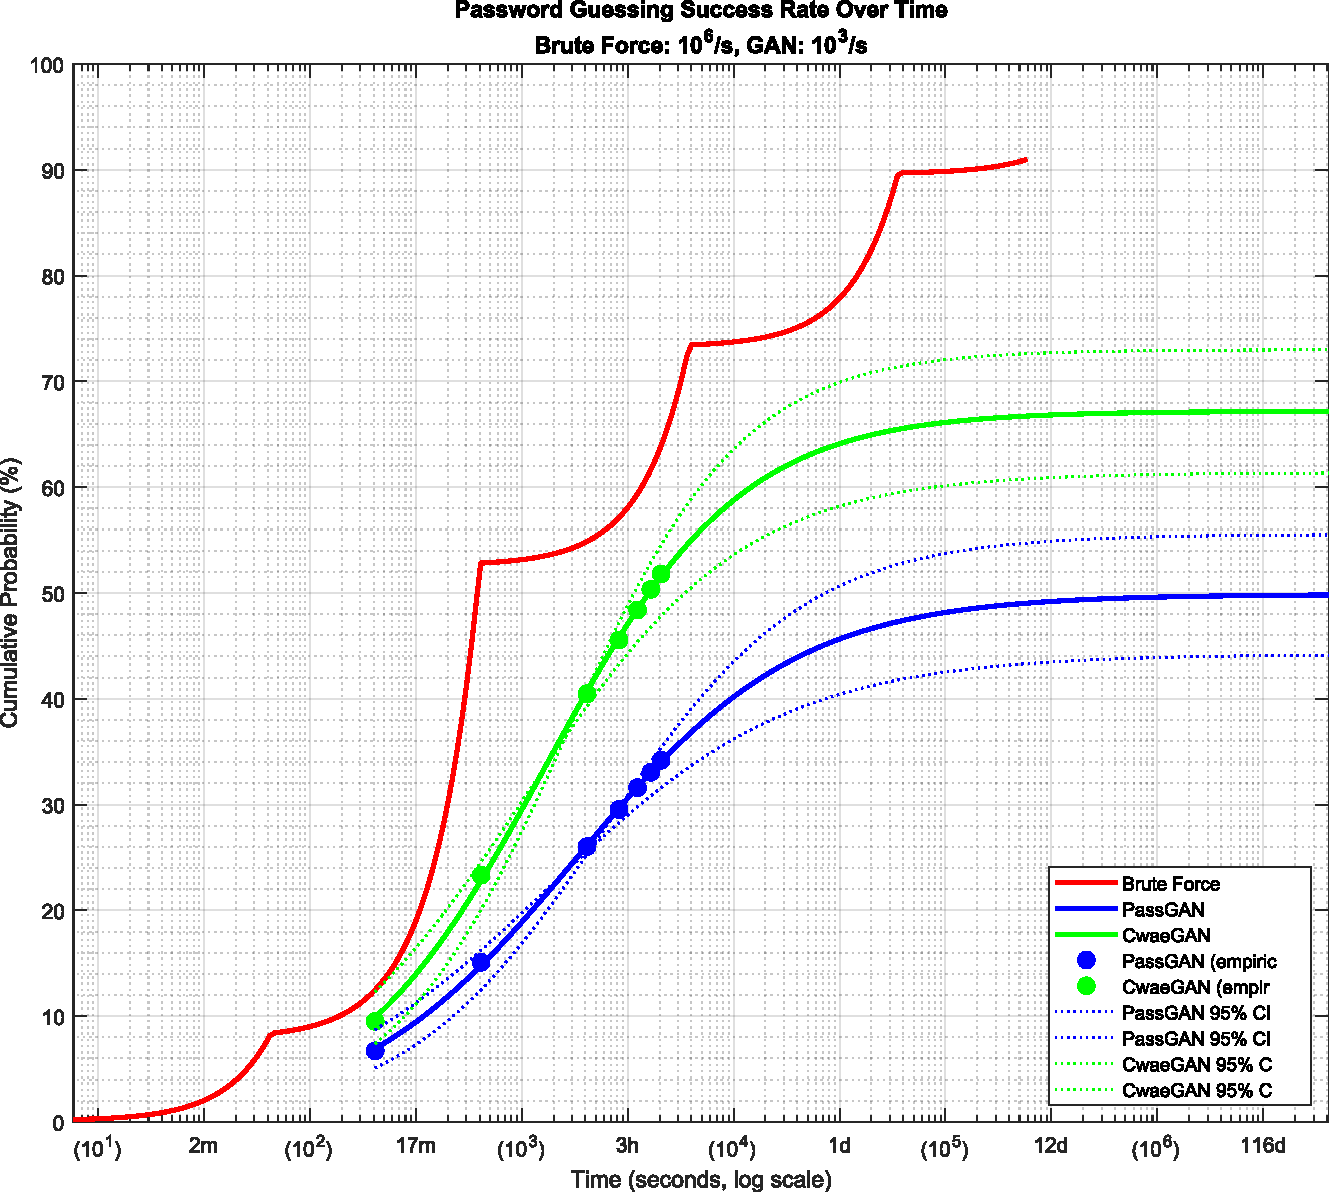
\includegraphics[scale=0.6]{figs/how_passwords/time_cdf.pdf}
    \caption{Calculating $F(N(t))$, incorporating both probability of guessing and the rate at which it happens gives us a more accurate view of the performance of password guessing algorithms. This framework demonstrates the utility of considering both generation quality and speed. \srcOwnFig}
    \label{fig:cracking-time}
\end{figure}

Figure~\ref{fig:cracking-time} shows our result using the same models as the number of guesses section. Here we assume the process is throttled by the number of candidates the GAN models are generating, i.e. $N(t) = \lambda t$, where $\lambda$ is the arrival rate and therefore the generation speed.

For our empirical analysis, we used the same dataset configurations as in the previous guessing probability evaluation - the RockYou password leak processed to contain passwords up to 10 characters. We measured the actual time taken to generate and process password guesses using both brute-force and GAN approaches across different hardware configurations.

The hashing rate $\mu$ is based on \hashcat benchmarks on consumer-level hardware. The hash rate is dependent on the hash function we are inverting and the hardware being used. Higher hash rate favours the brute-force method.

% \begin{enumerate}
% \item Despite lower raw generation rates, GAN models initially achieve faster crack times for common passwords due to their more intelligent probability distribution of guesses.
% \item For passwords beyond the 60th percentile of complexity, the brute-force method becomes more efficient due to its superior generation rate overwhelming the GANs' more targeted guessing strategy.
% \item The crossover point occurs at approximately 45 minutes of cracking time on our test hardware, after which brute-force methods consistently outperform the GAN approaches.
% \end{enumerate}

This empirical analysis supports our theoretical predictions about the relationship between generation rate, hash rate, and cracking success. It also highlights an important practical consideration: while sophisticated guessing strategies may be more efficient for common passwords, hardware-optimized can remain competitive and optimisation of the implementations should be considered a novel piece of work.

\subsection{Other Strategies and Parallelisation}

In the two-stage model considered in this chapter (candidate generation \(\rightarrow\) hash verification), the effective cracking throughput is determined by the bottleneck between the candidate generation rate \(\lambda\) and the hash-processing capability \(\mu\). Here, the application of more advanced queueing theory would be beneficial for understanding how scaling the number of workers would affect guessing rates. Moreover, future work could also incorporate cost and the economics of password guessing at scale. In Figures~\ref{fig:cracking-time}~and~\ref{fig:password-expected-guesses}, we assumed the attacker is not parallelising either \(\lambda\) or \(\mu\). The attacks are conducted on a consumer level hardware (internally the hashing might be parallelised at CPU or GPU level).

Increasing the number of generator or hashing workers changes the arrival process \(N(t)\) and consequently the expected time-to-crack derived earlier. Framing parallelism in this way allows formal comparison between algorithmic improvements (better candidate ranking) and systems improvements (higher \(\lambda\) or \(\mu\)).

For neural-network-based attacks, the system becomes constrained by the model’s candidate-generation rate rather than by the computational hashing throughput. Generating intelligent password candidates requires significantly more computational resources per guess than verifying them. In this scenario, we can scale the number of generators, optimise generation speed through model compression or quantisation techniques, or precompute candidates. Ultimately, the strategy to choose depends on the attacker’s intent, the type of neural network, and the target. There are leaked password dictionaries with billions of records already, so unless the neural network has better or more novel candidates, precomputing may not be useful.

When scaling the candidate-generation workers for neural networks, we can theoretically match or exceed the hashing rate $\mu$, but this approach faces practical limitations due to memory-bandwidth constraints, inter-processor communication overheads, and the inherently sequential nature of some neural network operations. However, parallelisation enables neural networks to reach their maximum potential, $M$, more quickly, without fundamentally altering their learning characteristics. Therefore, we would merely reach that asymptotic ceiling more quickly while preserving the underlying intelligence limitations of the model architecture.

For naive brute-force strategies, the hashing rate can be parallelised almost linearly, significantly improving $\mu$. This near-perfect parallel scaling gives brute-force approaches a significant advantage in highly parallel environments, potentially offsetting some of the intelligence-related benefits of neural approaches when sufficient computational resources are available.

Our work in this section remains valid when applying parallelisation techniques, and the approach we have taken enables us to reason effectively about parallelisation. Moreover, it prepares us to carry out future experiments using queueing theory, and even to consider the economics of password-guessing strategies.

% %\subsection{Queueing Model}
We model the process using a single server queue. The potential candidates are generated at near deterministic rate $\lambda$ and similarly the passwords are hashed and processed at near deterministic rate $\mu$. Therefore using Kendal's notation, the system is modelled as G/G/1. Let $\lambda(t)$ represent the arrival rate, and let $\mu(t)$ represent the hashing rate (this is typically referred to as the service rate). The utilization of our hashing server $H$ is:
\begin{equation}
    \rho = \frac{\lambda}{\mu}
\end{equation}

The utilization factor $\rho = \frac{\lambda}{\mu}$ must satisfy $\rho < 1$ for system stability, implying that the generation rate cannot exceed the processing capacity of the hashing function. 

\[
\rho = \lambda \, \mathbb{E}[S]
\]

The expected wait time in the system (queue and hashing) is given by the Kingman's approximation for our G/G/1 system.
\begin{equation}
    \mathbb{E}[W] = \frac{\rho}{1 - \rho} \cdot \frac{c_a^2 - c_s^2}{2} \cdot \mathbb{E}[S]
\end{equation}
The expected time in the system for a given password candidate:
\begin{equation}
    \mathbb{E}[T] = \mathbb{E}[S] + \mathbb{E}[W]
\end{equation}
\begin{equation}
    \mathbb{E}[T] = \left[ 1 + \frac{\rho}{1 - \rho} \cdot \frac{c_a^2 - c_s^2}{2} \right] \cdot \mathbb{E}[S]
\end{equation}
Based on, we can now calculate the expected number of password candidates in the system using Little's law:
\begin{equation}
    \mathbb{E}[N] = \lambda \mathbb{E}[T]
\end{equation}
\begin{equation}
    \mathbb{E}[N] = \rho + \frac{\rho^2(c_a^2 - c_s^2)}{2(1 - \rho)}
\end{equation}

Ideally we would like our server to be operating at maximum capacity, i.e. to maximise the resources available. This implies that our password generation should match the service rate of our server. However, we still want password candidates with high probability of inverting the hash function. So, a better measure of password guessing algorithm would be the expected time to crack--i.e. the expected time for an algorithm to invert the hash function. This takes into consideration the resources available to us and the probability distribution of an algorithm successfully guessing a password.

% \subsection{Resource Constraints and Optimization}
% 
% Let $C(t)$ represent the computational cost function:
% \[
% C(t) = c_g \int_0^t \lambda(s) \, ds + c_h \int_0^t \min\{\lambda(s), \mu(s)\} \, ds,
% \]
% where $c_g$ and $c_h$ are the unit costs for candidate generation and hashing, respectively.
% 
% The optimization problem can be formulated as:
% \begin{align*}
% \max_{\lambda(t)} & \quad F(N(T)) \\
% \text{subject to:} & \quad C(T) \leq B, \\
% & \quad \lambda(t) \geq 0, \\
% & \quad \int_0^T \lambda(t) \, dt \leq K,
% \end{align*}
% where $B$ represents the total computational budget and $K$ is the maximum number of allowable guesses.
% 
% To solve this optimization problem, we set up the Lagrangian:
% \[
% \mathcal{L} = F(N(T)) - \alpha \left( C(T) - B \right) - \gamma \left( \int_0^T \lambda(t) \, dt - K \right),
% \]
% where $\alpha \geq 0$ and $\gamma \geq 0$ are Lagrange multipliers.
% 
% Taking the functional derivative of $\mathcal{L}$ with respect to $\lambda(t)$, we obtain the necessary condition for optimality:
% \[
% \frac{\delta \mathcal{L}}{\delta \lambda(t)} = \frac{dF}{dN} \frac{dN}{d\lambda(t)} - \alpha \left( c_g + c_h \frac{d}{d\lambda(t)} \min\{\lambda(t), \mu(t)\} \right) - \gamma = 0.
% \]
% 
% The derivative $\frac{dN}{d\lambda(t)}$ depends on whether $\lambda(t) \leq \mu(t)$ or $\lambda(t) > \mu(t)$.
% 
% If $\lambda(t) < \mu(t)$:
% \[
% \min\{\lambda(t), \mu(t)\} = \lambda(t), \quad \frac{d}{d\lambda(t)} \min\{\lambda(t), \mu(t)\} = 1,
% \]
% so the derivative simplifies.
% 
% If $\lambda(t) > \mu(t)$:
% \[
% \min\{\lambda(t), \mu(t)\} = \mu(t), \quad \frac{d}{d\lambda(t)} \min\{\lambda(t), \mu(t)\} = 0.
% \]
% 
% Therefore, we need to consider these cases separately to derive the optimal control for $\lambda(t)$.

% \subsection*{Weibull Parameter Estimation}
% 
% Empirical studies, such as those involving PassGAN, have shown that password success probabilities can be approximated by the Weibull distribution. Given a success rate $p$ after $n$ guesses, the Weibull parameters can be determined by solving:
% \[
% p = F(n) = 1 - e^{-(n/\eta)^\beta}.
% \]
% 
% Taking the natural logarithm of both sides:
% \[
% \ln(1 - p) = -\left( \frac{n}{\eta} \right)^\beta.
% \]
% 
% Taking the logarithm again:
% \[
% \ln(-\ln(1 - p)) = \beta \ln n - \beta \ln \eta.
% \]
% 
% This linear relationship allows for estimation of $\beta$ and $\eta$ using linear regression on the transformed data, plotting $\ln(-\ln(1 - p))$ versus $\ln n$.



% \begin{itemize}[leftmargin=11pt]
% \item \textbf{\textsc{Generate.}} Given some input or some state, generate a single guess. Generators can have no input, a masked input, or even a full input. Methods, such as Deep Learning (DL) or Markov n-gram, can be applied to any of the generators. We will cover these specific methods later. Mask generators are covered in detail in \S\ref{chp5::sec::mask-attack}. The generation phase is crucial as it determines the quality and relevance of the guesses produced.
% 
% \item \textbf{\textsc{Filter.}} Generated guesses are further filtered if they do not meet certain criteria. The filter can be any function, such as rule-based filters (e.g., minimum length or required character sets). Effective filtering can reduce the search space and thus reduce the time it takes to guess a password. Filtering is often needed because the output of deep learning techniques could invalidate certain experimental conditions.
% 
% \item \textbf{\textsc{Guess.}} The final phase involves actually guessing the password with respect to some hash value. The filtered guesses are hashed using the appropriate algorithm (e.g. MD5, SHA-1) and compared against the target hash.
% \end{itemize}

% \subsection{Discussion and Future Works}
% 
% Our modelling of the process in this manner is the first of its kind and naturally we have begun this with a simple model. We foresee much more complex models that would incorporate different types of resources, queues, and even different types of incoming hash types. For example, one might prioritise MD5 hashes on GPU, bcrypt using FPGA or ASICs if such resources are available.